\documentclass[a4paper, 12pt]{article}
\usepackage[utf8]{inputenc}
\usepackage{graphicx}
\usepackage{geometry}
\usepackage{amsmath}
\usepackage{amssymb}
\usepackage{amsfonts}
\usepackage{float}
\usepackage{enumerate}
\usepackage{sectsty}
\usepackage{fancyhdr}
\usepackage{tikz}
\usepackage{gensymb}
\usepackage{hyperref}
\usepackage{siunitx}
\usepackage{xcolor}
\usepackage{multicol}
\usepackage{colortbl}
\usepackage{datetime}
\usepackage[english]{babel}
\usepackage{listings}
\usepackage{graphics}
\usepackage{caption}
\usepackage{subcaption}
\usepackage{booktabs}
\usepackage{array}
\usepackage{mdframed}
\usepackage{pgfgantt}
\usepackage{longtable}
\usetikzlibrary{shapes.geometric, arrows.meta, positioning, fit, backgrounds, calc}

% ---- Code listing style ----
\lstdefinestyle{bashstyle}{
    language=bash,
    basicstyle=\ttfamily\footnotesize,
    backgroundcolor=\color{gray!8},
    frame=single,
    rulecolor=\color{gray!60},
    breaklines=true,
    tabsize=2,
    captionpos=b,
    keywordstyle=\color{blue!70!black}\bfseries,
    commentstyle=\color{green!50!black},
    stringstyle=\color{red!70!black},
    numbers=left,
    numberstyle=\tiny\color{gray},
    stepnumber=1,
    numbersep=6pt,
    showstringspaces=false,
    morekeywords={conda, activate, python, cd, scp, ssh, source, wandb},
}
\lstset{style=bashstyle}

% ---- Coloured stage boxes ----
\newmdenv[
  backgroundcolor=blue!5,
  linecolor=blue!40,
  linewidth=1pt,
  roundcorner=4pt,
  innertopmargin=6pt,
  innerbottommargin=6pt,
]{stagebox}

\newmdenv[
  backgroundcolor=orange!5,
  linecolor=orange!50,
  linewidth=1pt,
  roundcorner=4pt,
  innertopmargin=6pt,
  innerbottommargin=6pt,
]{warnbox}

\newmdenv[
  backgroundcolor=green!5,
  linecolor=green!50,
  linewidth=1pt,
  roundcorner=4pt,
  innertopmargin=6pt,
  innerbottommargin=6pt,
]{successbox}

\geometry{top=2.5cm, bottom=2.5cm, right=2cm, left=2cm}
\pagestyle{fancy}
\rhead{Mini Forklift Automation}
\lhead{AIFARM ROBOTICS FACTORY}
\chead{}
\cfoot{Page \thepage}
\lfoot{AUTOBOTx LAB}
\rfoot{06.2026--09.2026}
\renewcommand{\headrulewidth}{1pt}
\renewcommand{\footrulewidth}{1pt}

\hypersetup{
    colorlinks=true,
    linkcolor=black,
    urlcolor=blue,
}

\title{\textbf{\LARGE Mini Forklift Automation}\\[0.4em]}
\author{\textbf{AIFARM Robotics Factory}\\Yin Chheanyun}
\date{\textbf{June 2026}}

\begin{document}

\begin{titlepage}
  \centering

  \includegraphics[width=5.0cm]{aifarm_logo.png}\\[0.5cm]

  {\Large\bfseries\sffamily AIFARM ROBOTICS FACTORY}\\[0.15cm]
  {\small\itshape Intelligent Robotics Research \& Development}\\[0.4cm]

  \noindent\rule{\linewidth}{1pt}\\[1.2cm]

  {\Huge\bfseries Mini Robot Forklift Automation}\\[0.4cm]
  {\Large\bfseries Prototype Development Proposal}\\[1.0cm]

  \noindent\rule{0.5\linewidth}{0.6pt}\\[1.0cm]

  \begin{tabular}{rl}
    \textbf{Author}         & Yin Chheanyun \\[0.3em]
    \textbf{Project}        & Mini Robot Forklift Automation Prototype \\[0.3em]
    \textbf{Platform}       & ROS2-Humble / Gazebo-Fortress / STM32 / Raspberry Pi 4B \\[0.3em]
    \textbf{Environment}    & \SI{2.0}{m} $\times$ \SI{2.0}{m} Indoor Arena \\[0.3em]
    \textbf{Date}           & June 2026 \\[0.3em]
    \textbf{Version}        & 1.0 \\
  \end{tabular}

  \vfill

  \noindent\rule{\linewidth}{1pt}\\[0.3cm]
  {\footnotesize\textit{Confidential --- AIFARM Robotics Factory Internal Document}}\\[0.1cm]
  {\footnotesize\textit{For internal research and development use only.}}\\[0.3cm]
  \noindent\rule{\linewidth}{2pt}
\end{titlepage}

\clearpage
\tableofcontents
\listoffigures
\listoftables
\newpage

%======================================================================
\section{Introduction}
%======================================================================

\subsection{Motivation}

Warehouse and small-scale factory intralogistics increasingly rely on
Autonomous Mobile Robots (AMRs) to move pallets and totes between fixed
storage, staging, and production locations without continuous human
supervision. Full-size industrial forklift AMRs are expensive to acquire,
difficult to modify, and impractical as a platform for iterative research
on navigation, docking, and fleet-coordination algorithms. The
\textbf{Mini Forklift AMR} closes this gap: it is a 1:10-scale, low-cost,
fully open research platform that reproduces the core behaviours of an
industrial pallet-handling AMR --- autonomous navigation, precision
docking, fork lifting, and multi-robot route coordination --- inside a
\SI{2.0}{m}\,$\times$\,\SI{2.0}{m} indoor arena.

The motivation for building this prototype is threefold:

\begin{enumerate}
    \item \textbf{Robotics research.} The platform provides a physical
    and simulated testbed for evaluating SLAM, localization, path
    planning, and precision-docking algorithms under realistic sensing
    noise and actuation constraints, at a fraction of the cost and risk
    of a full-scale vehicle.
    \item \textbf{Autonomous pallet transportation.} The system
    demonstrates the complete pick-and-drop workflow required by
    intralogistics automation: mission dispatch, navigation to a pallet
    location, marker-based alignment, lift engagement, and delivery to a
    drop location.
    \item \textbf{Fleet management and routing.} By combining a shared
    route graph with a traffic-arbitration layer, the platform is a
    proving ground for multi-robot coordination strategies used in
    industrial AGV/AMR fleets, in the spirit of VDA 5050-style
    graph-based routing (see \S\ref{sec:vda-lif}).
\end{enumerate}

\subsection{Scope of Work}

This document covers the complete development scope of the Mini Forklift
AMR prototype, from mechanical design through real-world deployment:

\begin{itemize}
    \item \textbf{Mechanical design} of the chassis, fork/lift
    mechanism, and drivetrain (\S\ref{sec:physical-specs}).
    \item \textbf{Embedded control} on STM32 microcontrollers for motor
    and lift actuation (\S\ref{sec:hardware-architecture}).
    \item \textbf{ROS 2 Humble software stack} running on a Raspberry Pi
    4B, covering perception, localization, navigation, docking, and task
    orchestration (\S\ref{sec:software-architecture}).
    \item \textbf{Simulation} of the robot and its environment in
    Gazebo Fortress, for both single- and multi-robot scenarios
    (\S\ref{sec:simulation}).
    \item \textbf{Precision docking} using ArUco fiducial markers for
    charging stations, pallet pick, and pallet drop operations
    (\S\ref{sec:precision-docking}).
    \item \textbf{Fleet routing} using a shared route graph and a
    traffic-management layer for multi-robot edge reservation
    (\S\ref{sec:vda-lif}).
    \item \textbf{Web dashboard} (Next.js, FastAPI, MongoDB) for fleet
    monitoring, control, and diagnostics (\S\ref{sec:web-dashboard}).
    \item \textbf{Real deployment} on the physical prototype, including
    the transition from simulated to physical sensing and control
    (\S\ref{sec:real-deployment}).
\end{itemize}

Sections~\ref{sec:testing}--\ref{sec:conclusion} evaluate the system
against measurable criteria, discuss current limitations, and outline
future work.

%======================================================================
\section{System Overview}
%======================================================================

\subsection{Physical Specifications}
\label{sec:physical-specs}

The Mini Forklift AMR is a compact, 1:10-scale reproduction of an
industrial counterbalance forklift. The current prototype dimensions are:

\begin{table}[H]
\centering
\caption{Mini Forklift physical dimensions.}
\label{tab:physical-dims}
\begin{tabular}{lccc}
\toprule
\textbf{Component} & \textbf{Length} & \textbf{Width} & \textbf{Height} \\
\midrule
Chassis      & \SI{200}{mm} & \SI{200}{mm} & \SI{300}{mm} \\
Fork         & \SI{150}{mm} & \SI{200}{mm} & \SI{250}{mm} \\
\bottomrule
\end{tabular}
\end{table}

\begin{table}[H]
\centering
\caption{Lift mechanism travel.}
\label{tab:lift-travel}
\begin{tabular}{lc}
\toprule
\textbf{Parameter} & \textbf{Value} \\
\midrule
Lift travel & \SI{0.15}{m} \\
\bottomrule
\end{tabular}
\end{table}

The mechanical structure is built from:

\begin{itemize}
    \item 3D-printed structural and bracket parts.
    \item Aluminium extrusion profiles for the mast/chassis frame.
    \item A belt-driven mechanism for fork lift actuation.
    \item Four drive wheels (differential or skid-steer drivetrain).
    \item A fork/lift carriage capable of \SI{0.15}{m} of vertical
    travel.
\end{itemize}

% Image suggestion:
% Photograph of the assembled prototype, or a dimensioned CAD/technical
% drawing showing chassis and fork envelope.

\begin{figure}[H]
    \centering
    \includegraphics[width=0.7\linewidth]{images/prototype_photo}
    \caption{Mini Forklift AMR prototype -- physical dimensions overview.}
    \label{fig:prototype_photo}
\end{figure}

\subsection{Hardware Architecture}
\label{sec:hardware-architecture}

The hardware is organized into three layers: a compute layer running the
ROS 2 software stack, a sensing layer providing perception and state
estimation inputs, and an embedded/actuation layer responsible for
low-level motor and lift control.

\subsubsection*{Computer Layer}

\begin{itemize}
    \item \textbf{Raspberry Pi 4B} -- the on-board robot computer,
    running ROS 2 Humble, the navigation/docking/task-management stack,
    and the web bridge.
    \item \textbf{Development PC} -- used for simulation (Gazebo
    Fortress), software development, remote monitoring (RViz2, rqt),
    and hosting the web dashboard front end during development.
\end{itemize}

\subsubsection*{Sensing Layer}

\begin{itemize}
    \item \textbf{RPLIDAR 2D} -- 2D laser scanner for SLAM mapping,
    AMCL localization, and Nav2 costmap obstacle observation.
    \item \textbf{IMU} -- provides angular velocity and linear
    acceleration for sensor fusion (extended Kalman filter).
    \item \textbf{Camera} -- RGB camera used for ArUco marker detection
    and pallet-vision object detection.
    \item \textbf{ToF sensor} -- short-range time-of-flight distance
    sensor used to support close-range docking and obstacle detection.
\end{itemize}

\subsubsection*{Embedded / Actuation Layer}

\begin{itemize}
    \item \textbf{STM32F401} -- main embedded controller, interfacing
    with the Raspberry Pi over serial and coordinating actuation
    commands.
    \item \textbf{STM32F103} -- dedicated DC motor control
    microcontroller.
    \item \textbf{L298N / BTS7960} -- H-bridge motor driver stages for
    the drivetrain.
    \item \textbf{Stepper motor / servo} -- actuates the fork lift
    mechanism.
\end{itemize}

% Image suggestion:
% Full hardware architecture diagram (compute / sensing / embedded
% layers and their interconnects).

\begin{figure}[H]
    \centering
    \includegraphics[width=\linewidth]{images/system_architecture}
    \caption{Hardware architecture of the Mini Forklift AMR prototype.}
    \label{fig:system_architecture}
\end{figure}

\subsection{Pick-and-Drop Workflow}

The core mission behaviour of the robot is the pick-and-drop workflow,
orchestrated by the task-management layer (\S\ref{sec:ros2-stack}). A
single mission request is expanded into an ordered sequence of
navigation, docking, and lift steps:

\begin{stagebox}
\begin{center}
\begin{tabular}{c}
\textbf{Mission Request} \\
$\downarrow$ \\
Navigate to Pickup \\
$\downarrow$ \\
Dock \\
$\downarrow$ \\
ArUco / Camera Alignment \\
$\downarrow$ \\
Lift Fork \\
$\downarrow$ \\
Undock \\
$\downarrow$ \\
Navigate to Drop \\
$\downarrow$ \\
Dock \\
$\downarrow$ \\
Lower Fork \\
$\downarrow$ \\
Undock \\
$\downarrow$ \\
\textbf{Mission Complete}
\end{tabular}
\end{center}
\end{stagebox}

Each stage maps onto a concrete ROS 2 action call: navigation stages use
Nav2's \texttt{NavigateToPose}, docking stages use the docking server's
\texttt{DockRobot}/\texttt{UndockRobot} actions with ArUco-derived pose
feedback, and lift stages use \texttt{SetLiftHeight}. This decomposition
is implemented independently (with some duplication, discussed in
\S\ref{sec:ros2-stack}) by both \texttt{forklift\_task\_manager} and
\texttt{forklift\_docking}'s pallet-dock workflow action.

% Image suggestion:
% State-machine diagram of the pick-and-drop workflow, or a sequence
% diagram of the task manager driving navigation/docking/lift actions.

\begin{figure}[H]
    \centering
    \includegraphics[width=\linewidth]{images/pick_drop_workflow}
    \caption{Pick-and-drop mission workflow state machine.}
    \label{fig:pick_drop_workflow}
\end{figure}

%======================================================================
\section{Software Architecture}
\label{sec:software-architecture}
%======================================================================

\subsection{ROS 2 Humble Stack}
\label{sec:ros2-stack}

The software stack is organized as a layered pipeline from the operator
(web dashboard) down to the physical actuators, mirroring the ROS 2
workspace layout (17 packages under \texttt{miniforklift\_ws/src}):

\begin{stagebox}
\begin{center}
\begin{tabular}{c}
Web Dashboard \\
$\downarrow$ \\
Web Bridge (\texttt{forklift\_web\_bridge}: REST, rosbridge WebSocket, web video server) \\
$\downarrow$ \\
Mission Manager (\texttt{forklift\_mission\_manager}) \\
$\downarrow$ \\
Task Manager (\texttt{forklift\_task\_manager}) \\
$\downarrow$ \\
Navigation / Docking / Lift Controller \\
(\texttt{forklift\_navigation}, \texttt{forklift\_docking}, \texttt{forklift\_controller}) \\
$\downarrow$ \\
ROS 2 Hardware Interface \\
$\downarrow$ \\
STM32 + Sensors + Motors
\end{tabular}
\end{center}
\end{stagebox}

\begin{itemize}
    \item \textbf{ROS 2} provides the underlying pub/sub, service, and
    action communication middleware that connects every node in the
    stack.
    \item \textbf{TF2} maintains the coordinate-frame tree
    (\texttt{map} $\to$ \texttt{odom} $\to$ \texttt{base\_link} $\to$
    sensor frames), used by localization, navigation, and marker-based
    docking alike.
    \item \textbf{Nav2} supplies the navigation stack: global/local
    costmaps, planner server, controller server, behaviour-tree
    navigator, and recovery behaviours.
    \item \textbf{SLAM Toolbox} builds the occupancy grid map from
    RPLIDAR scans during the mapping phase (\S\ref{sec:mapping}).
    \item \textbf{AMCL} (or an equivalent particle-filter localizer)
    localizes the robot against a previously built map once mapping is
    complete.
    \item \textbf{Controller Server} executes the local trajectory
    controller (MPPI/DWB, \S\ref{sec:navigation}) that converts the
    global plan into velocity commands.
    \item \textbf{Costmaps} (global and local) fuse LiDAR and inflation
    layers to represent static and dynamic obstacles for planning and
    control.
    \item \textbf{Route Server} (\texttt{nav2\_route}) plans and tracks
    routes over a static graph of nodes and edges, used for the VDA
    LiF-style routing layer (\S\ref{sec:vda-lif}).
    \item \textbf{rosbridge} exposes ROS 2 topics/services/actions over
    a WebSocket for the web dashboard.
    \item \textbf{web\_video\_server} streams the on-board camera feed
    to the web dashboard over HTTP.
\end{itemize}

\begin{figure}[H]
    \centering
    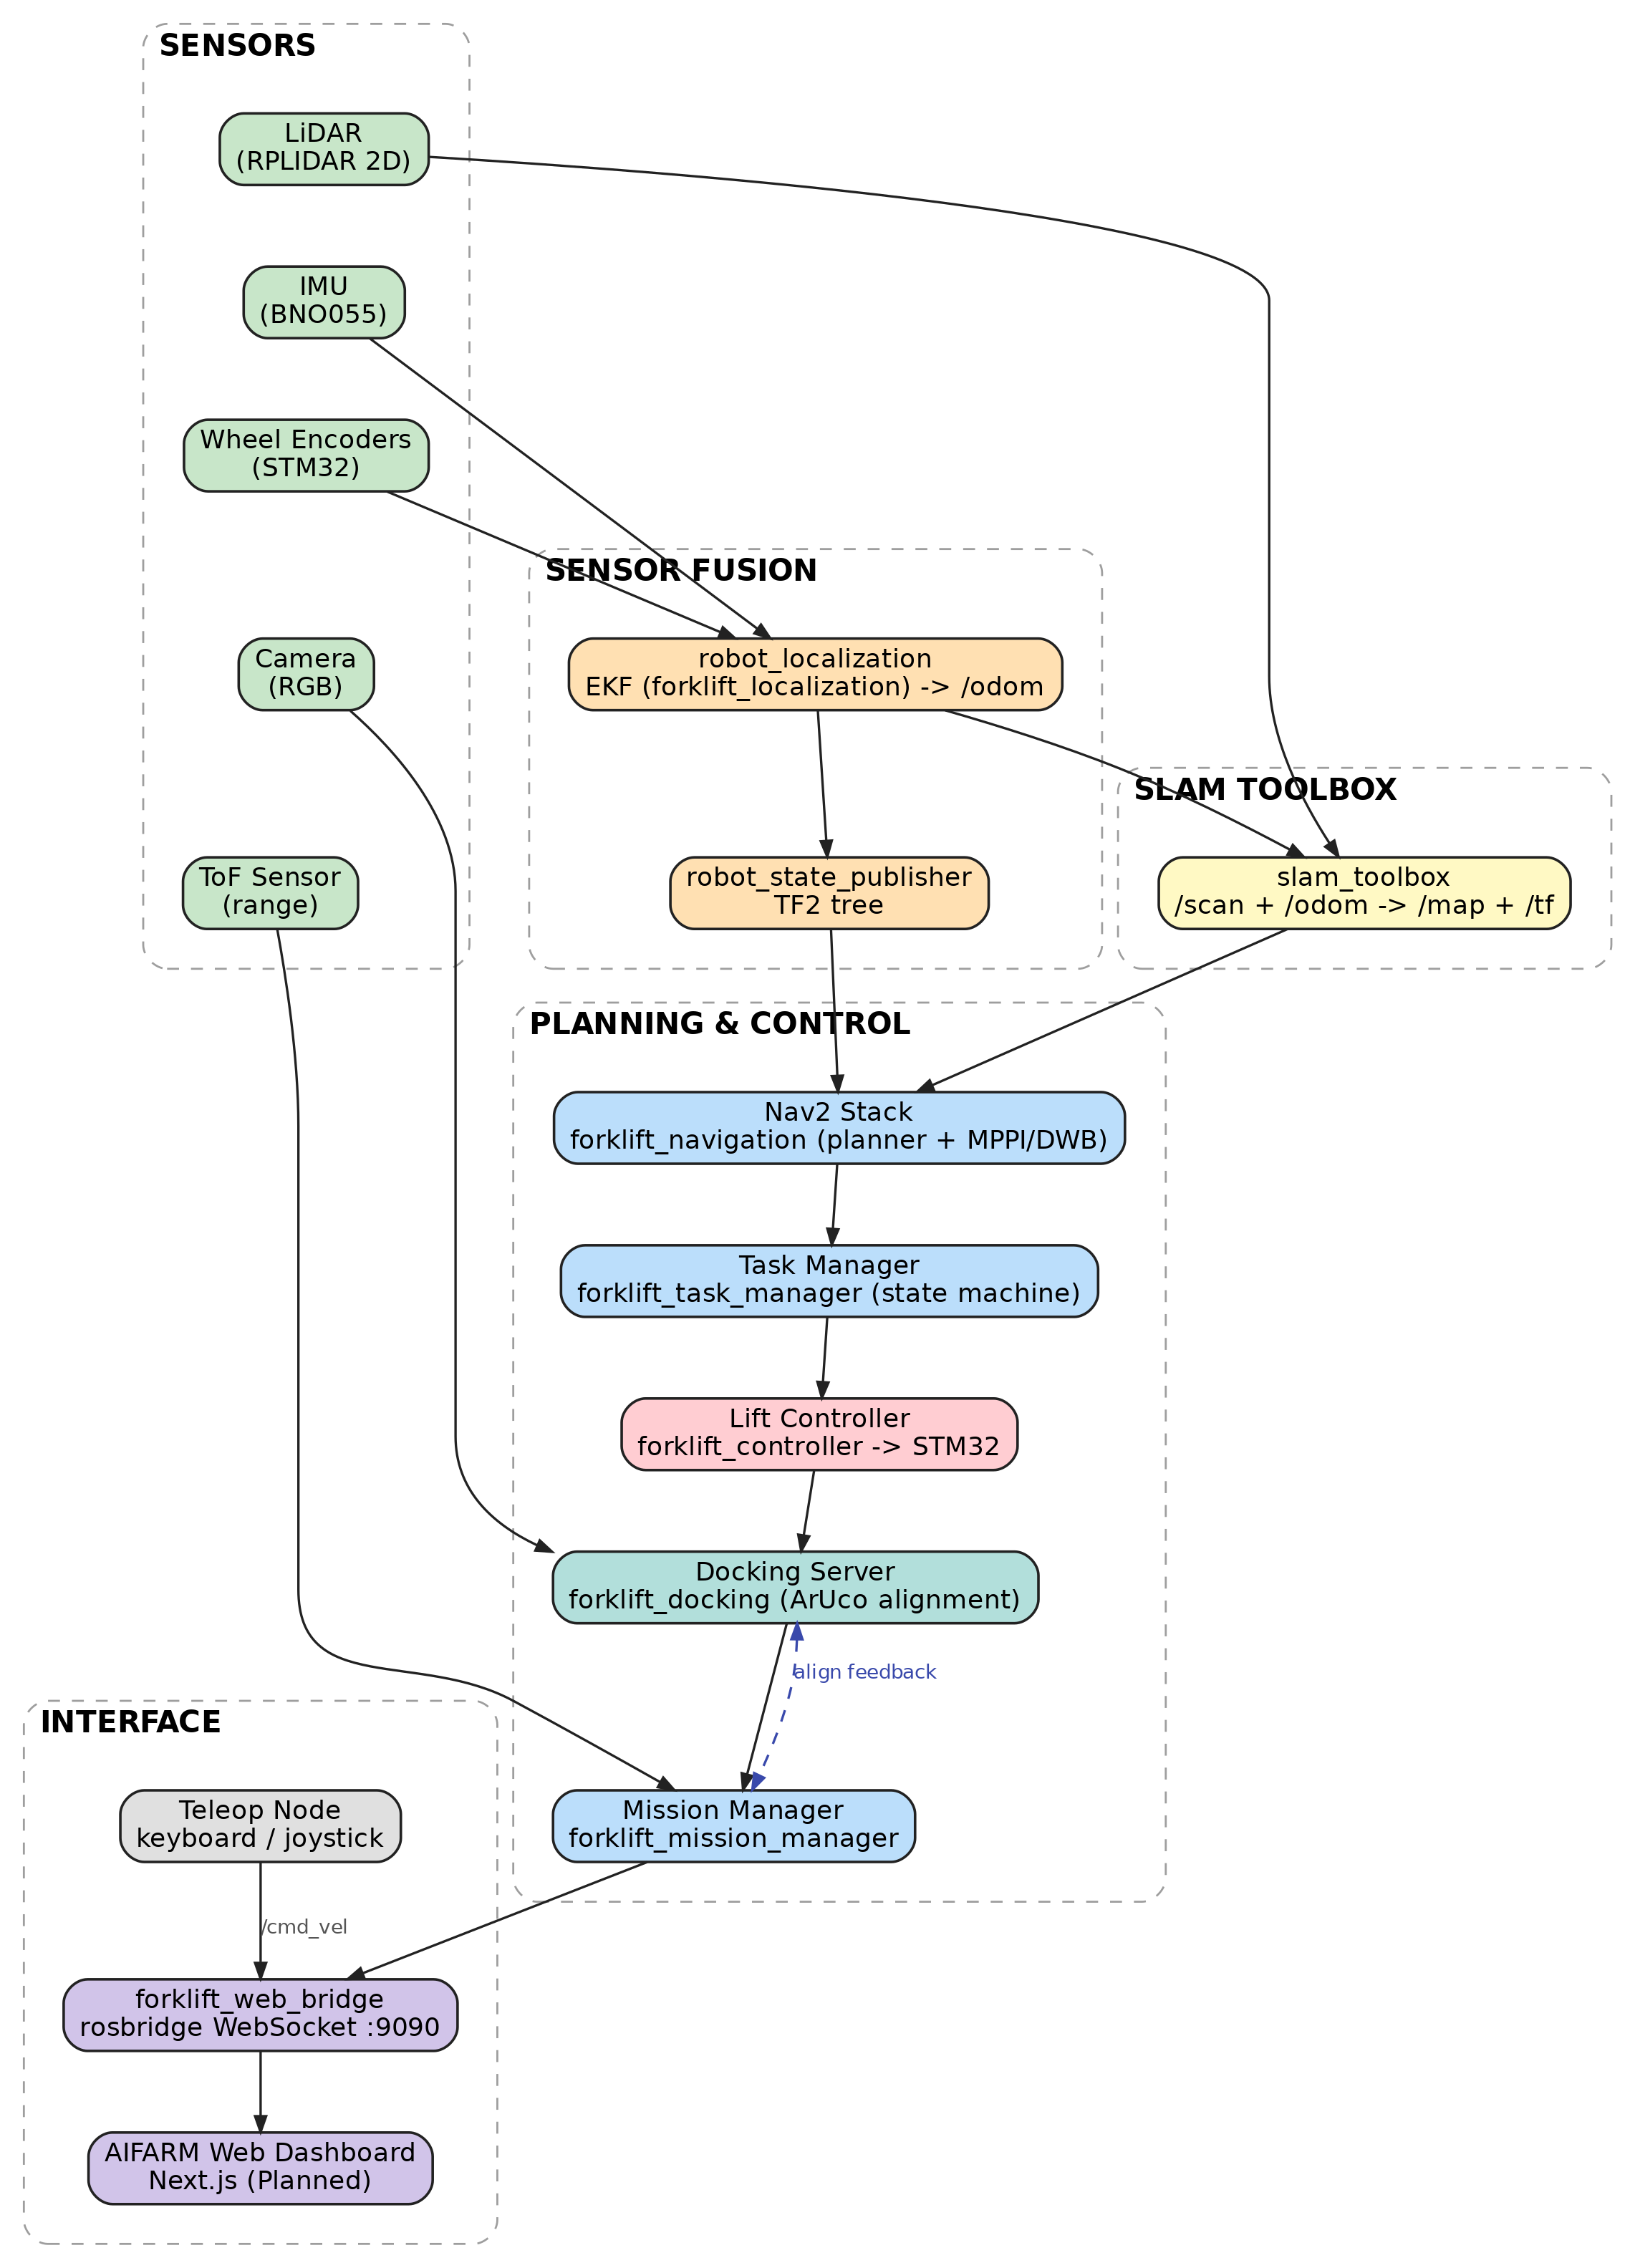
\includegraphics[width=\linewidth]{images/software_architecture}
    \caption{ROS 2 software architecture of the Mini Forklift AMR: the
      vertical pipeline (blue) shows the command/control path from the
      web dashboard down to the embedded controller; orange boxes and
      dashed arrows show the supporting ROS 2 middleware and sensing
      inputs consumed by the Navigation and Docking layers.}
    \label{fig:software_architecture}
\end{figure}

\subsection{Mapping}
\label{sec:mapping}

The occupancy grid map used for localization and navigation is built
offline (or online) using SLAM Toolbox, consuming raw 2D laser scans from
the RPLIDAR sensor:

\begin{stagebox}
\begin{center}
\textbf{RPLIDAR} $\rightarrow$ \textbf{SLAM Toolbox} $\rightarrow$ \textbf{Occupancy Grid Map}
\end{center}
\end{stagebox}

SLAM Toolbox performs scan matching and pose-graph optimization to
produce a consistent 2D occupancy grid of the \SI{2.0}{m}\,$\times$\,\SI{2.0}{m}
arena, which is then serialized and reused by AMCL/Nav2 for subsequent
autonomous operation.

% Image suggestion:
% Screenshot of the SLAM Toolbox map of the test arena (RViz2 occupancy
% grid view).

\begin{figure}[H]
    \centering
    \includegraphics[width=0.8\linewidth]{images/slam_map}
    \caption{Occupancy grid map of the test arena generated by SLAM Toolbox.}
    \label{fig:slam_map}
\end{figure}

\subsection{Navigation}
\label{sec:navigation}

Autonomous navigation is provided by the Nav2 stack, configured through
\texttt{forklift\_navigation}. The pipeline consists of:

\begin{itemize}
    \item \textbf{Localization} -- AMCL (or an EKF-fused estimate from
    \texttt{forklift\_localization}, see \S\ref{sec:real-deployment})
    provides the robot's pose in the \texttt{map} frame.
    \item \textbf{Global planning} -- the planner server computes a
    collision-free path from the current pose to the goal over the
    global costmap.
    \item \textbf{Local control} -- the controller server tracks the
    global path in real time, issuing velocity commands while reacting
    to the local costmap.
    \item \textbf{Costmaps} -- global and local costmaps combine static
    map data, LiDAR obstacle observations, and an inflation layer to
    keep the robot at a safe distance from obstacles.
    \item \textbf{Controller Server / MPPI / DWB} -- the local
    trajectory controller plugin; MPPI (Model Predictive Path
    Integral) and DWB (Dynamic Window local planner) are both supported
    Nav2 controller plugins and may be selected per deployment.
    \item \textbf{Pure Pursuit} -- an alternative lightweight
    path-tracking controller used for simpler point-to-point motion.
    \item \textbf{Goal Checker} -- determines when the robot is close
    enough (position and heading tolerance) to a goal to be considered
    "arrived."
    \item \textbf{Recovery} -- Nav2 recovery behaviours (e.g.\ spin,
    back-up, clear costmap) triggered when the controller or planner
    fails to make progress.
\end{itemize}

Key tuning parameters that shape navigation behaviour include:

\begin{table}[H]
\centering
\caption{Key Nav2 tuning parameters.}
\label{tab:nav2-params}
\begin{tabular}{ll}
\toprule
\textbf{Parameter} & \textbf{Effect} \\
\midrule
Linear velocity (max/min) & Maximum/minimum forward speed \\
Angular velocity (max/min) & Maximum/minimum turning rate \\
Acceleration limits & Rate of change of linear/angular velocity \\
Lookahead distance & Pure Pursuit / path-tracking horizon \\
Heading tolerance & Allowed heading error before rotation is considered complete \\
Goal (position) tolerance & Allowed distance error to consider a goal reached \\
Obstacle inflation radius / cost scaling & Aggressiveness of obstacle avoidance \\
\bottomrule
\end{tabular}
\end{table}

The controller is configured to rotate in place to the target heading
before committing to forward motion, which improves tracking accuracy on
the tight \SI{2.0}{m}\,$\times$\,\SI{2.0}{m} arena used for testing:

\begin{stagebox}
\begin{center}
\begin{tabular}{c}
Rotate to target heading \\
$\downarrow$ \\
Reach heading tolerance \\
$\downarrow$ \\
Move forward \\
$\downarrow$ \\
Continue path tracking
\end{tabular}
\end{center}
\end{stagebox}

% Image suggestion:
% RViz2 screenshot showing a planned global path, local costmap, and the
% robot tracking the path.

\begin{figure}[H]
    \centering
    \includegraphics[width=0.8\linewidth]{images/navigation_rviz}
    \caption{Nav2 path planning and tracking, visualized in RViz2.}
    \label{fig:navigation_rviz}
\end{figure}

\subsection{ArUco Marker}

Precision alignment for docking relies on ArUco fiducial marker
detection, implemented in \texttt{forklift\_aruco}:

\begin{stagebox}
\begin{center}
\textbf{Camera} $\rightarrow$ \textbf{ArUco Detection} $\rightarrow$ \textbf{Marker ID} $\rightarrow$ \textbf{Pose Estimation} $\rightarrow$ \textbf{TF} $\rightarrow$ \textbf{Precision Alignment}
\end{center}
\end{stagebox}

The camera feed is processed to detect ArUco markers placed at charging
stations, pallet pick locations, and pallet drop locations. Each
detected marker yields a marker ID (used to distinguish target
locations) and a 6-DoF pose estimate relative to the camera, which is
published as a TF transform and consumed by the docking layer
(\S\ref{sec:precision-docking}) to compute the final alignment
correction.

% Image suggestion:
% Camera image with an ArUco marker detected and its axes/pose overlay
% drawn.

\begin{figure}[H]
    \centering
    \includegraphics[width=0.6\linewidth]{images/aruco_detection}
    \caption{ArUco marker detection and pose estimation from the on-board camera.}
    \label{fig:aruco_detection}
\end{figure}

\subsection{Precision Docking}
\label{sec:precision-docking}

\texttt{forklift\_docking} implements four docking modes, all sharing a
common approach-align-verify-undock structure:

\begin{table}[H]
\centering
\caption{Precision docking modes.}
\label{tab:docking-modes}
\begin{tabular}{ll}
\toprule
\textbf{Mode} & \textbf{Purpose} \\
\midrule
Charging & Align to a charging-station marker for battery charging \\
Station & Align to a general-purpose waypoint/station marker \\
Pallet Pick & Align to a pallet-pick marker before lifting \\
Pallet Drop & Align to a pallet-drop marker before lowering \\
\bottomrule
\end{tabular}
\end{table}

Each docking mode follows the same behavioural sequence:

\begin{enumerate}
    \item \textbf{Approach} -- navigate to a staging pose near the
    target marker.
    \item \textbf{Alignment} -- use the ArUco-derived pose
    (\S\ref{sec:navigation} preceding) to servo the robot into final
    position and heading.
    \item \textbf{Tolerance check} -- verify the robot is within
    configured position and heading tolerance of the target.
    \item \textbf{Success detection} -- confirm docking success (pose
    within tolerance, held for a stability window).
    \item \textbf{Timeout / recovery} -- abort and retry (or back off
    and re-approach) if alignment is not achieved within a timeout.
    \item \textbf{Undocking} -- reverse away from the dock along a safe
    retreat path once the docking operation (charge, pick, drop) is
    complete.
\end{enumerate}

% Image suggestion:
% Docking workflow / state-machine figure showing approach, align,
% verify, and undock states.

\begin{figure}[H]
    \centering
    \includegraphics[width=\linewidth]{images/docking_workflow}
    \caption{Precision docking workflow.}
    \label{fig:docking_workflow}
\end{figure}

\subsection{VDA LiF Routing}
\label{sec:vda-lif}

Multi-robot route coordination is implemented on top of Nav2's
\texttt{nav2\_route} package, using a statically defined graph of nodes
and edges describing valid travel lanes in the arena, in the spirit of
VDA 5050-style, line-following (LiF) graph routing.

\begin{itemize}
    \item \textbf{Route graph} -- a set of nodes (waypoints/stations)
    and edges (directed lanes) describing the drivable layout of the
    environment.
    \item \textbf{Nodes} -- fixed poses (pickup points, drop points,
    charging stations, intersections).
    \item \textbf{Edges} -- directed, weighted connections between
    nodes that the robot may traverse.
    \item \textbf{Route Server} -- the \texttt{nav2\_route} server that
    loads the route graph and exposes route planning/tracking actions.
    \item \textbf{Route planning} -- computing a sequence of graph
    edges from the robot's current node to a goal node.
    \item \textbf{Route tracking} -- following the planned sequence of
    edges, handing off to the local controller for each edge segment.
    \item \texttt{/route\_graph} -- the published/loaded route graph
    used by the route server.
    \item \texttt{/compute\_route} -- service/action to plan a route
    without executing it.
    \item \texttt{/compute\_and\_track\_route} -- action to plan and
    immediately execute (track) a route.
\end{itemize}

On top of the single-robot route server, \texttt{forklift\_traffic\_manager}
adds fleet-wide arbitration: a \texttt{traffic\_manager\_node} grants or
denies exclusive claims on shared route-graph edges via a
\texttt{reserve\_edge} service, and pushes dynamic edge-cost adjustments
to each robot's route server so that a route already claimed by one
robot is penalized (and avoided) in another robot's route planning.

\begin{stagebox}
\begin{center}
\textbf{Route Graph} $\rightarrow$ \textbf{Route Server} $\rightarrow$ \textbf{Navigation} $\rightarrow$ \textbf{Robot}
\end{center}
\end{stagebox}

\begin{warnbox}
\textbf{Terminology note:} the routing layer described here follows the
\emph{graph-based routing philosophy} of VDA 5050 / LiF (line-following)
AGV standards -- a shared node/edge graph, route planning, and
edge-level traffic arbitration -- but it does \emph{not} currently
implement the literal VDA 5050 Order/State JSON message schema over
MQTT. Full VDA 5050 protocol compliance is tracked as future work
(\S\ref{sec:future-work}).
\end{warnbox}

% Image suggestion:
% Screenshot of the route graph (nodes/edges) as authored in a VDA LiF
% graph editor, overlaid on the arena map.

\begin{figure}[H]
    \centering
    \includegraphics[width=0.8\linewidth]{images/route_graph}
    \caption{Route graph (nodes and edges) used by the Route Server.}
    \label{fig:route_graph}
\end{figure}

%======================================================================
\section{Web Dashboard}
\label{sec:web-dashboard}
%======================================================================

The web dashboard is the human-machine interface for fleet monitoring
and manual control. It communicates with the ROS 2 stack exclusively
through \texttt{forklift\_web\_bridge}, which exposes a REST API, a
rosbridge WebSocket endpoint, and a video streaming endpoint.

\begin{stagebox}
\begin{center}
\begin{tabular}{c}
Next.js \\
$\downarrow$ \\
FastAPI / WebSocket \\
$\downarrow$ \\
ROS Bridge \\
$\downarrow$ \\
ROS 2
\end{tabular}
\end{center}
\end{stagebox}

\subsubsection*{Technologies}

\begin{itemize}
    \item \textbf{Next.js} -- front-end framework for the dashboard UI.
    \item \textbf{MongoDB} -- persistent storage for mission history,
    task logs, and configuration.
    \item \textbf{FastAPI} -- back-end API service layer.
    \item \textbf{rosbridge} -- WebSocket bridge exposing ROS 2
    topics/services/actions to the web layer.
    \item \textbf{web\_video\_server} -- HTTP MJPEG streaming of the
    on-board camera feed.
    \item \textbf{MQTT} -- \emph{Planned}; not yet implemented.
\end{itemize}

\subsubsection*{Dashboard Functions}

\begin{itemize}
    \item Dashboard -- system overview and quick status.
    \item Fleet Dashboard -- multi-robot overview.
    \item Live Map -- real-time occupancy grid and robot pose.
    \item Robot Status -- battery, connectivity, and operational state.
    \item Camera -- live camera stream view.
    \item Navigation -- goal dispatch and path visualization.
    \item Patrol -- repeating waypoint patrol control.
    \item Relocate -- manual pose (re-)initialization.
    \item Task -- single-task dispatch and monitoring.
    \item Mission -- multi-task mission dispatch and monitoring.
    \item Manual Control -- teleoperation.
    \item Diagnostics -- aggregated system diagnostics view.
    \item Sensor status -- per-sensor health/status view.
    \item Controller tuning -- runtime adjustment of navigation
    controller parameters.
\end{itemize}

\begin{warnbox}
\textbf{Status:} the Next.js/MongoDB/FastAPI web dashboard front end is
\textbf{Planned / Future Work}. The ROS 2 back end it will consume
(\texttt{forklift\_web\_bridge}: REST API, rosbridge WebSocket, and
web\_video\_server endpoints) is implemented and operational; the
dashboard UI itself has not yet been built in this workspace.
\end{warnbox}

% Image suggestion:
% Screenshots of the main dashboard view and the navigation / manual
% control pages, once the front end exists.

\begin{figure}[H]
    \centering
    \includegraphics[width=0.8\linewidth]{images/dashboard_main}
    \caption{Web dashboard -- main overview page (Planned).}
    \label{fig:dashboard_main}
\end{figure}

\begin{figure}[H]
    \centering
    \includegraphics[width=0.8\linewidth]{images/dashboard_control}
    \caption{Web dashboard -- navigation / manual control page (Planned).}
    \label{fig:dashboard_control}
\end{figure}

%======================================================================
\section{Simulation Implementation}
\label{sec:simulation}
%======================================================================

Simulation is performed in Gazebo Fortress, using \texttt{forklift\_gazebo}
and \texttt{forklift\_description} to reproduce the robot model and test
arena.

\subsection{Single Robot}

The single-robot simulation reproduces the full stack end-to-end in a
simulated environment:

\begin{itemize}
    \item \textbf{Robot model} -- URDF/xacro description of the
    chassis, wheels, and fork/lift mechanism, with simulated sensor
    plugins for the RPLIDAR, IMU, and camera.
    \item \textbf{World} -- a \SI{2.0}{m}\,$\times$\,\SI{2.0}{m} test
    arena world matching the physical test environment.
    \item \textbf{Sensors} -- simulated RPLIDAR, IMU, and camera
    publishing to the same topics used on the real robot.
    \item \textbf{Navigation} -- the same Nav2 configuration used on
    hardware, driven against the simulated sensors.
    \item \textbf{Localization} -- AMCL/EKF localization against the
    simulated map and simulated odometry/IMU.
    \item \textbf{Docking} -- ArUco markers placed in the simulated
    world for docking validation.
    \item \textbf{Lift simulation} -- simulated actuation of the fork
    lift joint through \texttt{SetLiftHeight}.
\end{itemize}

% Image suggestion:
% Gazebo Fortress screenshot of the single robot in the simulated test
% arena.

\begin{figure}[H]
    \centering
    \includegraphics[width=0.8\linewidth]{images/gazebo_single_robot}
    \caption{Single-robot simulation in Gazebo Fortress.}
    \label{fig:gazebo_single_robot}
\end{figure}

\subsection{Multiple Robots}

Multi-robot simulation reuses the single-robot model, spawned multiple
times under distinct ROS 2 namespaces:

\begin{stagebox}
\begin{center}
\texttt{/forklift1} \quad \texttt{/forklift2} \quad \texttt{/forklift3}
\end{center}
\end{stagebox}

Each namespace carries its own TF tree, sensor topics, and navigation
stack instance, while the traffic-management layer
(\S\ref{sec:vda-lif}) arbitrates shared route-graph edges across all
spawned robots to prevent collisions at intersections and shared lanes.

% Image suggestion:
% Gazebo Fortress screenshot of multiple forklift robots operating
% simultaneously in the shared simulated arena.

\begin{figure}[H]
    \centering
    \includegraphics[width=0.8\linewidth]{images/gazebo_multi_robot}
    \caption{Multi-robot simulation in Gazebo Fortress.}
    \label{fig:gazebo_multi_robot}
\end{figure}

\subsection{Simulation Functions}

The following functions are exercised in simulation prior to
deployment on hardware:

\begin{itemize}
    \item Simple navigation (point-to-point goal dispatch).
    \item Charging docking.
    \item Station docking.
    \item Pallet pick docking.
    \item Pallet drop docking.
    \item Routing (multi-node route planning and tracking).
\end{itemize}

% Image suggestion:
% One screenshot per simulated test above (navigation, each docking
% mode, and routing).

\begin{figure}[H]
    \centering
    \includegraphics[width=0.8\linewidth]{images/sim_navigation_test}
    \caption{Simulation test -- simple navigation.}
    \label{fig:sim_navigation_test}
\end{figure}

\begin{figure}[H]
    \centering
    \includegraphics[width=0.8\linewidth]{images/sim_docking_test}
    \caption{Simulation test -- precision docking (charging / station / pallet pick / pallet drop).}
    \label{fig:sim_docking_test}
\end{figure}

\begin{figure}[H]
    \centering
    \includegraphics[width=0.8\linewidth]{images/sim_routing_test}
    \caption{Simulation test -- route planning and tracking.}
    \label{fig:sim_routing_test}
\end{figure}

%======================================================================
\section{Real Robot Deployment}
\label{sec:real-deployment}
%======================================================================

Deployment to the physical prototype follows the simulation validation
described in \S\ref{sec:simulation}, replacing simulated sensors and
actuators with their physical counterparts while reusing the same ROS 2
software stack.

\begin{itemize}
    \item \textbf{Raspberry Pi 4B} -- runs ROS 2 Humble and the full
    navigation/docking/task-management stack on-board.
    \item \textbf{ROS 2 Humble} -- identical node graph to simulation,
    with hardware driver nodes replacing Gazebo sensor/actuator
    plugins.
    \item \textbf{RPLIDAR} -- physical 2D LiDAR driver node replacing
    the simulated LiDAR plugin.
    \item \textbf{IMU} -- physical IMU driver, subject to real sensor
    noise and drift not present in simulation.
    \item \textbf{Camera} -- physical camera driver for ArUco detection
    and pallet vision.
    \item \textbf{ToF} -- physical time-of-flight sensor for close-range
    docking support.
    \item \textbf{STM32} -- embedded firmware executing motor and lift
    commands received from the Raspberry Pi over serial.
    \item \textbf{Motor drivers} -- L298N/BTS7960 driving the physical
    DC drive motors.
    \item \textbf{DC motors} -- physical drivetrain actuation.
    \item \textbf{Lift actuator} -- physical stepper/servo-driven fork
    lift mechanism.
    \item \textbf{Communication} -- serial link between Raspberry Pi and
    STM32 for actuator commands and sensor feedback.
    \item \textbf{Calibration} -- camera intrinsic/extrinsic calibration
    (see \texttt{calib.yaml}/\texttt{calib.npz} in the workspace),
    LiDAR-to-base-link extrinsics, and IMU bias calibration.
    \item \textbf{TF} -- physical sensor frame transforms must match
    the URDF used in simulation for consistent navigation behaviour.
    \item \textbf{Navigation tuning} -- Nav2 parameters
    (\S\ref{sec:navigation}) re-tuned against real sensor noise,
    wheel slip, and actuation latency.
    \item \textbf{Safety testing} -- validation of the safety layer
    (\texttt{forklift\_safety}: obstacle monitoring, protective field,
    speed zones, emergency stop) before autonomous operation on
    hardware.
\end{itemize}

\begin{table}[H]
\centering
\caption{Simulation system vs. real robot system.}
\label{tab:sim-vs-real}
\begin{tabular}{lll}
\toprule
\textbf{Aspect} & \textbf{Simulation System} & \textbf{Real Robot System} \\
\midrule
Sensors & Gazebo plugins & Physical RPLIDAR / IMU / Camera / ToF \\
Actuation & Simulated joints/wheels & STM32 + motor drivers + DC motors \\
Localization noise & Idealized/parametrized & Real sensor noise, drift, slip \\
Communication & Internal ROS 2 graph & Serial link (Pi $\leftrightarrow$ STM32) \\
Safety & Not required & \texttt{forklift\_safety} layer required \\
Timing & Simulated clock, deterministic & Real-time constraints, jitter \\
\bottomrule
\end{tabular}
\end{table}

\begin{warnbox}
The safety layer (\texttt{forklift\_safety}) is implemented but is
\textbf{not currently included in the default bringup launch}; it must
be launched explicitly. Autonomous operation on the physical robot
should not be performed without the safety layer active.
\end{warnbox}

% Image suggestion:
% Photographs of the physical robot, internal wiring/electronics, and
% real-world navigation/docking test runs.

\begin{figure}[H]
    \centering
    \includegraphics[width=0.8\linewidth]{images/real_robot_photo}
    \caption{Physical Mini Forklift AMR prototype.}
    \label{fig:real_robot_photo}
\end{figure}

\begin{figure}[H]
    \centering
    \includegraphics[width=0.8\linewidth]{images/wiring_diagram}
    \caption{Electrical wiring: Raspberry Pi, STM32, drivers, and sensors.}
    \label{fig:wiring_diagram}
\end{figure}

\begin{figure}[H]
    \centering
    \includegraphics[width=0.8\linewidth]{images/real_navigation_test}
    \caption{Real-robot navigation and docking test.}
    \label{fig:real_navigation_test}
\end{figure}

%======================================================================
\section{Testing and Evaluation}
\label{sec:testing}
%======================================================================

The following measurable criteria are used to evaluate system
performance. Where measurements have not yet been collected, the value
is marked \textbf{TBD}.

\begin{table}[H]
\centering
\caption{Navigation performance evaluation criteria.}
\label{tab:eval-navigation}
\begin{tabular}{lcc}
\toprule
\textbf{Metric} & \textbf{Target} & \textbf{Measured} \\
\midrule
Navigation success rate & TBD & TBD \\
Position error (goal) & TBD & TBD \\
Heading error (goal) & TBD & TBD \\
Navigation time (per run) & TBD & TBD \\
\bottomrule
\end{tabular}
\end{table}

\begin{table}[H]
\centering
\caption{Docking performance evaluation criteria.}
\label{tab:eval-docking}
\begin{tabular}{lcccc}
\toprule
\textbf{Docking Mode} & \textbf{Success Rate} & \textbf{Position Error} & \textbf{Heading Error} & \textbf{Time to Dock} \\
\midrule
Charging     & TBD & TBD & TBD & TBD \\
Station      & TBD & TBD & TBD & TBD \\
Pallet Pick  & TBD & TBD & TBD & TBD \\
Pallet Drop  & TBD & TBD & TBD & TBD \\
\bottomrule
\end{tabular}
\end{table}

\begin{table}[H]
\centering
\caption{Mission and system-level evaluation criteria.}
\label{tab:eval-mission}
\begin{tabular}{lc}
\toprule
\textbf{Metric} & \textbf{Measured} \\
\midrule
Mission completion time (pick-to-drop) & TBD \\
Lift positioning accuracy & TBD \\
Multi-robot operation (no collisions, edges arbitrated correctly) & TBD \\
Route execution (planned vs. actual path deviation) & TBD \\
\bottomrule
\end{tabular}
\end{table}

\begin{warnbox}
No experimental measurements have been recorded at the time of writing
this document. All numerical results above are placeholders (\textbf{TBD})
to be filled in once controlled test campaigns are run in both
simulation and on the physical prototype.
\end{warnbox}

%======================================================================
\section{Limitations and Future Work}
\label{sec:future-work}
%======================================================================

\begin{itemize}
    \item \textbf{Sensor limitations.} The 2D RPLIDAR cannot detect
    obstacles outside its scan plane (e.g.\ overhanging obstacles or
    low obstacles below the scan height); the ToF sensor has a limited
    field of view and range suitable only for close-range docking
    assistance.
    \item \textbf{Docking accuracy.} Vision-based ArUco alignment is
    sensitive to lighting conditions, marker occlusion, and camera
    calibration drift; systematic docking-accuracy measurements are
    required (\S\ref{sec:testing}).
    \item \textbf{Lift mechanism.} The belt/stepper-driven lift
    currently has no closed-loop position feedback beyond open-loop
    step counting; repeatability under load has not been
    characterized.
    \item \textbf{Hardware safety.} The \texttt{forklift\_safety}
    package is implemented but not wired into the default bringup
    launch; a hardware emergency-stop circuit independent of software
    is recommended before unattended operation.
    \item \textbf{Multi-robot coordination.} Traffic arbitration
    currently reserves individual graph edges; more advanced
    intersection management, deadlock avoidance, and priority
    scheduling remain future work.
    \item \textbf{Payload limitations.} Maximum pallet/payload mass has
    not yet been characterized against lift torque and drivetrain
    traction.
    \item \textbf{Real warehouse testing.} All testing to date is
    confined to the \SI{2.0}{m}\,$\times$\,\SI{2.0}{m} indoor arena;
    validation in a larger, more representative warehouse-like
    environment is future work.
    \item \textbf{Depth-camera docking.} Adding a depth camera would
    improve close-range docking robustness beyond monocular ArUco
    pose estimation.
    \item \textbf{Better pallet detection.} The YOLOv11-based
    \texttt{pallet\_vision} detector exists but is not yet integrated
    into the main docking/task pipeline (which currently relies on
    ArUco markers only); integrating learned pallet detection is
    future work.
    \item \textbf{ToF lift feedback.} Using the ToF sensor (or an
    additional one) for closed-loop lift height feedback is planned.
    \item \textbf{Emergency-stop system.} A dedicated, hardware-level
    emergency-stop system (button + watchdog, independent of the
    software safety stack) is planned.
    \item \textbf{Fleet scheduling.} Mission/task scheduling across
    multiple robots (beyond per-edge traffic arbitration) is future
    work.
    \item \textbf{VDA 5050 integration.} Full VDA 5050 protocol
    compliance (Order/State JSON messages over MQTT) is planned; the
    current routing layer implements the graph-routing concept but not
    the wire protocol (\S\ref{sec:vda-lif}).
\end{itemize}

%======================================================================
\section{Conclusion}
\label{sec:conclusion}
%======================================================================

The Mini Forklift AMR prototype integrates mechanical design, embedded
motor/lift control, and a full ROS 2 Humble software stack into a
complete, research-oriented autonomous pallet-handling platform. The
system demonstrates autonomous navigation via Nav2 and SLAM Toolbox,
precision docking via ArUco marker detection across four docking modes
(charging, station, pallet pick, pallet drop), and multi-robot route
coordination via a shared route graph with edge-level traffic
arbitration. The stack has been validated in single- and multi-robot
Gazebo Fortress simulation and is being brought onto the physical
Raspberry Pi 4B / STM32 prototype, with a web dashboard back end
(\texttt{forklift\_web\_bridge}) already operational ahead of the
planned Next.js/MongoDB/FastAPI front end.

The platform's main capabilities can be summarized as: (1) a complete
pick-and-drop mission workflow orchestrated end-to-end from a single
mission request; (2) a tuned Nav2 navigation stack with configurable
local controllers; (3) marker-based precision docking with defined
tolerance, timeout, and recovery behaviour; (4) a route-graph-based
fleet routing layer with traffic arbitration; and (5) a layered software
architecture that cleanly separates perception, navigation, docking,
task orchestration, and human-machine interfacing. The limitations and
future work identified in \S\ref{sec:future-work} -- most notably
closed-loop lift feedback, integrated pallet detection, a hardware
emergency-stop system, and full VDA 5050 protocol compliance -- define
the roadmap toward a warehouse-representative deployment of the
platform.

\end{document}
